\section{引言}

同策略蒸馏（OPD）~\citep{agarwal2024policy,gu2024minillm} 将强教师模型的推理与生成能力迁移至较小的学生模型。与离线蒸馏 \citep{kim-rush-2016-sequence} 或监督微调不同，它利用教师模型在学生自生成轨迹上的逐 token 监督进行训练，从而在长序列上降低曝光偏差。目前，OPD 已成为前沿实验室中大型语言模型（LLM）后训练的标准步骤，包括思维机器 \citep{lu2025onpolicydistillation}、GLM \citep{zeng2026glm} 以及 DeepSeek \citep{xu2026deepseek}。

标准的OPD \citep{agarwal2024policy} 需要在每个生成的 token 处获取教师模型的完整分布，这对现代大模型而言代价过高，因为其词表大小可达 250K 个 token，导致每条序列的开销随词表大小和回溯长度而增长。因此，实际训练系统通常采用稀疏教师接口，即在每一步仅返回教师模型的 Top-$k$ 个 token 及其概率，以及采样 token \citep{zhang2026ema,huang2026tail} 的概率。我们将通过此类接口训练得到的 OPD 称为 \textbf{稀疏 OPD}。问题在于被忽略的尾部从未被观测到：直接基于 Top-$k$ 支撑集定义的目标函数，无论是通过截断或规范化 \citep{zhu2026many}，还是将被忽略的质量聚合到一个“幽灵 token”中 \citep{anshumann-etal-2025-sparse,huang2026tail}，都只是全词表反向 Kullback-Leibler (rKL) 目标函数的代理，且会引入系统性梯度偏差（图~\ref{fig:estimator-anatomy}(b)）。

偏差可以与方差进行权衡：与其将目标函数收缩至观测到的支持集，另一类方法保留全词表的rKL目标，并从稀疏的负载中估计其梯度，保持\textbf{无偏但噪声较大}。然而，现有的估计量未能充分挖掘这一负载。在极端情况下，采样token的OPD \citep{gu2024minillm,lu2025onpolicydistillation} 仅查询回滚token的得分，由于单样本蒙特卡罗估计导致梯度方差严重（图~\ref{fig:estimator-anatomy}(b)）。在另一端，具有Top-$k$ 访问的方法则利用不足：标量基准变体如vOPD \citep{oh2026kl} 将头部简化为一个脱离的基准，而非解析地评估其逐token梯度（表~\ref{tab:mechanism}），而混合方案如\citet{zhang2026ema}（我们称之为头精确尾采样，HETS）虽然精确计算头部，却将尾部修正视为完全未知，尽管已知其总质量。因此，每次尾部命中必须补偿全部被忽略的质量，引入巨大的梯度尖峰；即使头部覆盖率达到98.4\%，一个30K token的推理轨迹也包含460--470次此类尖峰，每优化器步数上千次（第~\ref{sec:train_dynamics}节）。

因此，从业者不得不在有偏目标与不稳定梯度之间做出选择，这导致采样token的OPD和HETS在训练初期达到峰值后逐渐退化（第~\ref{sec:math-opd}节）。

\begin{figure}[t]
\centering
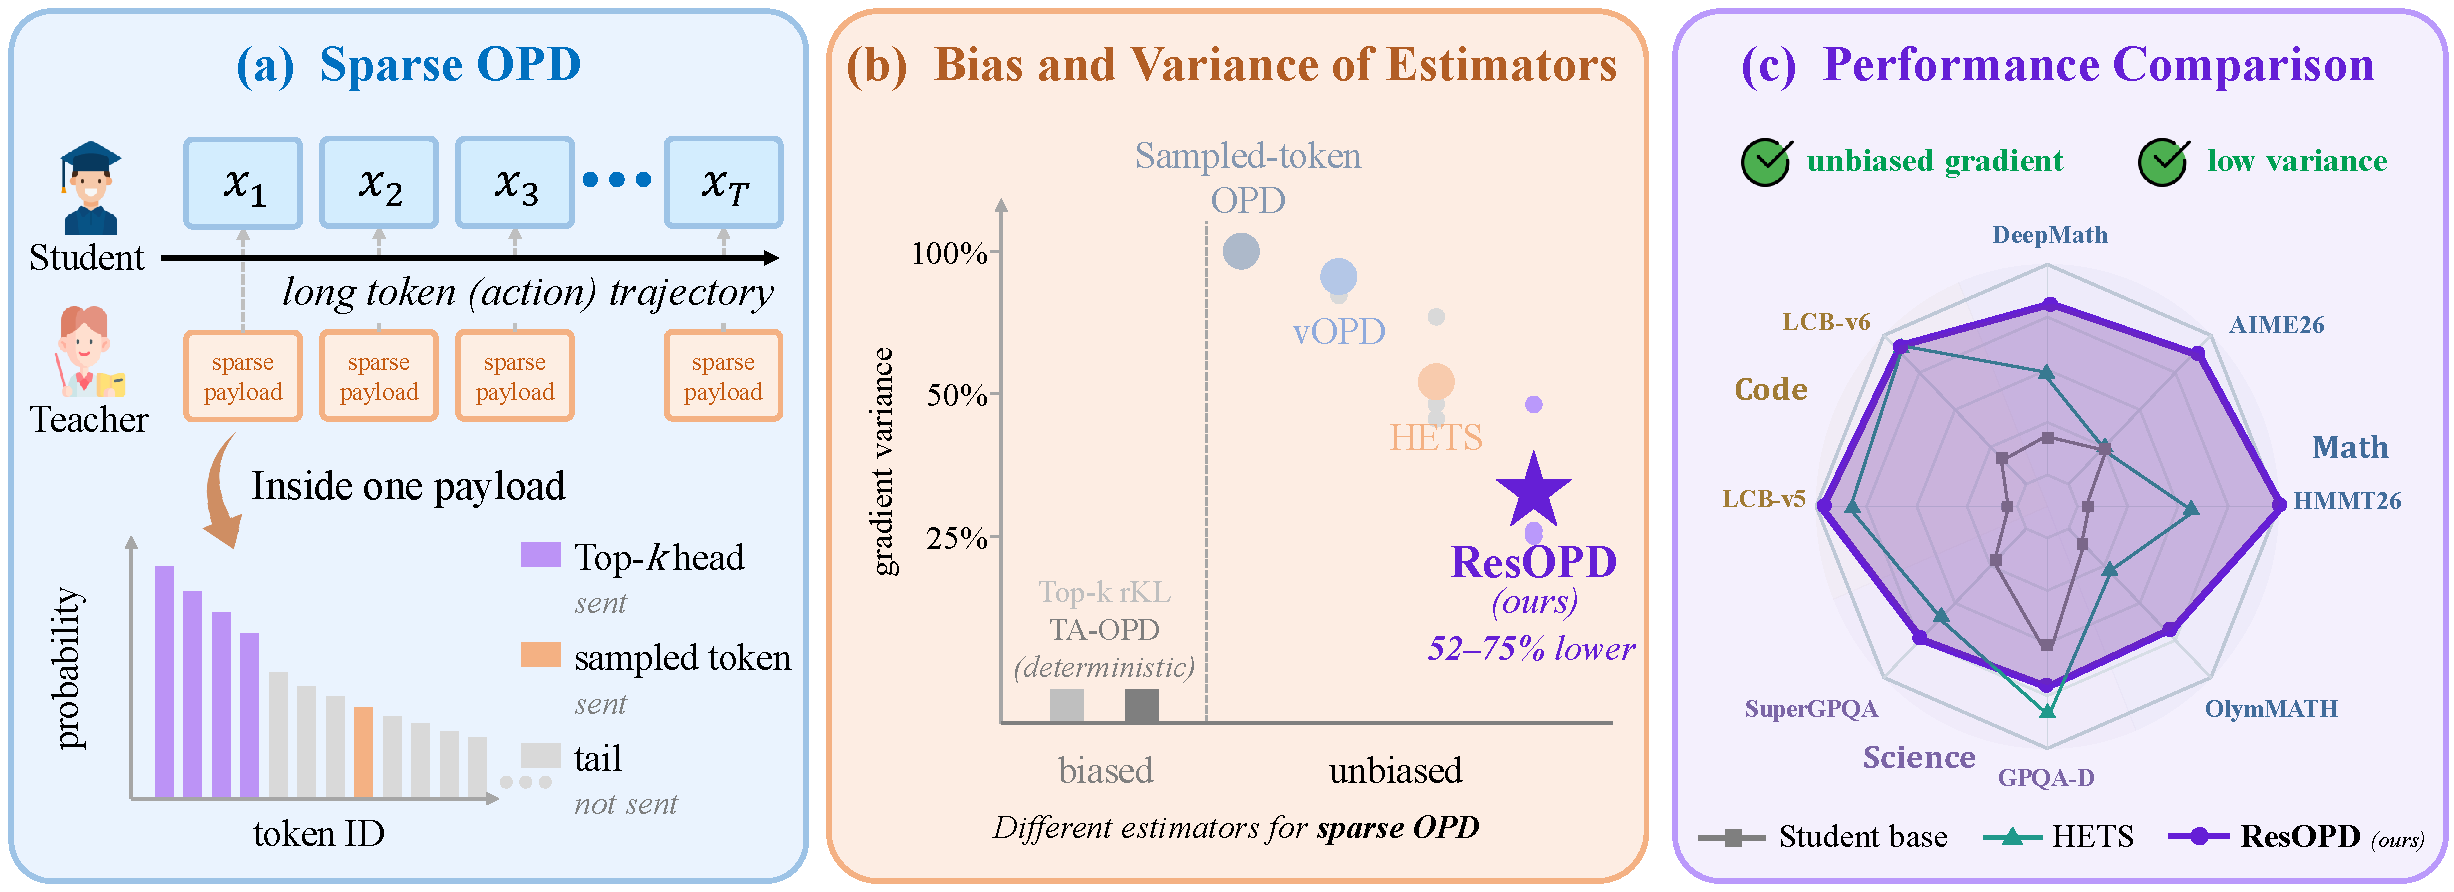
\includegraphics[width=1.0\textwidth]{figs/teaser_v21.pdf}
\caption{(a) 稀疏 OPD：教师模型仅发送 Top-$k$ 头部概率和采样 token 得分，尾部分布未被观测。(b) 偏差 vs. 方差权衡：虽然确定性 Top-$k$ 替代品存在系统性梯度偏差，但 ResOPD 提供了无偏梯度估计量并显著降低了梯度方差。(c) 下游评估：雷达图显示了数学、编程和科学领域的基准得分；尽管相对秩因任务而异，但 ResOPD 实现了最佳整体性能。}
\label{fig:estimator-anatomy}
\vspace{-4mm}
\end{figure}

为解决这一权衡，我们从梯度估计量的角度分析稀疏的OPD。我们首先证明，任何精确评估头部、添加由学生尾部质量加权的前缀相关控制向量，并在尾部命中时进行修正的估计量，对于全词表rKL梯度是无偏的，其中HETS是控制向量为零的特例（第~\ref{subsec:cfr}节）。我们的协方差-迹分解表明，方差分为一个与尾部采样不变的项和一个与控制向量到真实尾部均值距离成比例的事件间项。这解释了HETS的梯度尖峰现象：其零控制在每次命中时都需承担完整的尾部均值代价，而任何能更好预测该均值的控制向量均可严格降低方差。关键的是，头部之外的残差质量定义了一个粗粒度伪token \citep{anshumann-etal-2025-sparse,huang2026tail}，其解析梯度可作为可计算的尾部均值预测器。基于此，我们提出\textit{\textbf{O}n-\textbf{P}olicy \textbf{D}istillation with Tail \textbf{Res}idualization}（ResOPD）：每一步它计算$(k+1)$-路粗粒度分布的精确梯度，仅在尾部命中时添加微小残差修正（图~\ref{fig:framework}(a)）。所得估计量在保持相同稀疏教师负载的同时，被证明是无偏的。

我们在两种情景下评估了 ResOPD。在确切的冻结前缀审计中，通过枚举每个下一个 token 的动作，ResOPD 在 Top-$4$ 反馈下相较于采样 token 的 OPD 降低了 52--75\% 的梯度协方差迹，优于 HETS 和一个与载荷匹配的 vOPD 基准（表~\ref{tab:mechanism}）。在从 Qwen3.5-27B 到 Qwen3.5-4B 的端到端蒸馏中，它在四个数学推理基准上取得了所评估的稀疏 OPD 基准中的最高平均得分，相较于相同载荷下的 HETS 高出 4.40 分（表~\ref{tab:math-terminal}），且其相对于 HETS 的平均优势在所有测试的支持大小 $k\in\{1,4,16,32\}$ 下均保持一致，差距较小（表~\ref{tab:topk-breakdown}）。

我们的贡献如下：  
(1) \textbf{稀疏OPD的有偏与方差分析。} 我们证明了截断、重归一化以及停止系数的Top-$k$  rKL目标函数均为全词表目标函数的有偏替代，我们推导出一种协方差-迹分解，将尾部采样方差与事件间方差分离。该分解给出了粗粒度尾部控制相较于HETS降低方差的确切条件，并提出一个包含两类控制的家族，其中HETS、ResOPD以及同期的SC-TA \citep{huang2026tail} 均可作为特例。  
(2) \textbf{ResOPD估计量。} 我们提出一种估计量，将全词表rKL梯度分解为一个在每一步精确计算的$(k+1)$ -路粗粒度项，该部分基于Top-$k$ 的有效负载和残余尾部质量，以及仅在回放token落入尾部时才应用的尾部内部残差修正。该估计量在同策略采样下无偏，且无需额外的教师查询或前向传播。  
(3) \textbf{实验验证。} 通过确切的冻结前缀梯度审计及端到端蒸馏设置，我们表明ResOPD降低了梯度协方差，减少了训练过程中的在线残差矩，并在下游任务中提升了相对于所评估稀疏OPD基准的准确率。
